\documentclass[12pt,a4paper]{report}
\usepackage[italian]{babel}
\usepackage{newlfont}
\textwidth=450pt\oddsidemargin=0pt
\usepackage{amsmath}
\usepackage{amssymb}
\usepackage{amsthm}
\usepackage{xcolor}
\usepackage{listings}
\usepackage{tikz}
\usepackage{xspace}
\usepackage{indentfirst}
\graphicspath{ {./images/} }

\definecolor{dkgreen}{rgb}{0,0.6,0}
\definecolor{gray}{rgb}{0.5,0.5,0.5}
\definecolor{mauve}{rgb}{0.58,0,0.82}


\lstset{frame=tb,
  language=Java,
  aboveskip=3mm,
  belowskip=3mm,
  showstringspaces=false,
  columns=fullflexible,
  basicstyle={\small\ttfamily},
  numbers=left,
  numberstyle=\tiny\color{gray},
  keywordstyle=\color{blue},
  commentstyle=\color{dkgreen},
  stringstyle=\color{mauve},
  breaklines=true,
  breakatwhitespace=true,
  tabsize=1
}
\setlength\parindent{0pt}

\begin{document}
\begin{titlepage}
\begin{center}
{{\Large{\textsc{Alma Mater Studiorum $\cdot$ Universit\`a di
Bologna}}}} \rule[0.1cm]{15.8cm}{0.1mm}
\rule[0.5cm]{15.8cm}{0.6mm}
{\small{\bf SCUOLA DI SCIENZE\\
Corso di Laurea in Informatica }}
\end{center}
\vspace{15mm}

\begin{center}
{\LARGE{\bf Title thesis:}}\\
\vspace{3mm}
{\LARGE{\bf Subtitle thesis}}\\
\end{center}
\vspace{40mm}
\par
\noindent
\begin{minipage}[t]{0.47\textwidth}
{\large{\bf Relatore:\\
Chiar.mo Prof.\\
Maurizio Gabbrielli\\
\\
Correlatori:\\
Dott.\\
Stefano Pio Zingaro\\
Saverio Giallorenzo\\
}}
\end{minipage}
\hfill
\begin{minipage}[t]{0.47\textwidth}\raggedleft
{\large{\bf Presentata da:\\
Luca Genova}}
\end{minipage}
\vspace{20mm}
\begin{center}
{\large{\bf Sessione II\\%inserire il numero della sessione in cui ci si laurea
Anno Accademico 2020/2021}}%inserire l'anno accademico a cui si è iscritti
\end{center}
\end{titlepage}


\chapter*{Sommario}
Il Machine Learning è un sottoinsieme dell'intelligenza artificiale (AI) che si occupa di creare sistemi che apprendono o migliorano le performance in base ai dati che utilizzano. Intelligenza artificiale è un termine generico e si riferisce a sistemi o macchine che imitano l'intelligenza umana.\\
Definire in maniera semplice le caratteristiche e le applicazioni del machine learning non è sempre possibile, visto che questo ramo è molto vasto e prevede differenti modalità, tecniche e strumenti per essere realizzato. Inoltre, le differenti tecniche di apprendimento e sviluppo degli algoritmi danno vita ad altrettante possibilità di utilizzo che allargano il campo di applicazione dell’apprendimento automatico rendendone difficile una definizione specifica. Si può tuttavia dire che quando si parla di machine learning si parla di differenti meccanismi che permettono a una macchina intelligente di migliorare le proprie capacità e prestazioni nel tempo. La macchina, quindi, sarà in grado di imparare a svolgere determinati compiti migliorando, tramite l’esperienza, le proprie capacità, le proprie risposte e funzioni.\\
Alla base dell’apprendimento automatico ci sono una serie di differenti algoritmi che, partendo da nozioni primitive, sapranno prendere una specifica decisione piuttosto che un’altra o effettuare azioni apprese nel tempo.\\
L'obiettivo di questa tesi è rispondere alla domanda: \emph{Si possono autogenerare dei modelli?}\\
Per arrivare alla risposta ho analizzato in letteratura due casi studio, al fine di tirare fuori i relativi workflow per arrivare alla generalizzazione. Infatti è stato applicato un approccio bottom-up, partendo dai casi studio specifici fino alla generalizzazione.\\
I casi studio in questione sono:
\begin{itemize}
    \item AI in radiology
    \item Demand forecasting
\end{itemize}
Alla fine scopriremo che non sempre è possibile, dipende fortemente dall'applicazione del modello.

\tableofcontents

\chapter{Introduzione}
\par
Le prime sperimentazioni per la realizzazione di macchine intelligenti risalgono agli inizi degli anni Cinquanta del Novecento, quando alcuni matematici e statistici iniziarono a pensare di utilizzare i metodi probabilistici per realizzare macchine che potessero prendere decisioni proprio tenendo conto delle probabilità di accadimento di un evento. Il primo grande nome legato al machine learning è sicuramente quello di Alan Turing, che ipotizzò la necessità di realizzare algoritmi specifici per realizzare macchine in grado di apprendere. In quegli stessi anni, anche gli studi sull’intelligenza artificiale, sui sistemi esperti e sulle reti neurali vedevano momenti di grossa crescita alternati da periodi di abbandono, causati soprattutto dalle molte difficoltà riscontrate nelle possibilità di realizzazione dei diversi sistemi intelligenti, nella mancanza di sussidi economici e dallo scetticismo che circondava spesso chi provava a lavorarci. A partire dagli anni Ottanta, una serie di interessanti risultati ha portato alla rinascita di questo settore della ricerca: una rinascita che è stata resa possibile da nuovi investimenti nel settore. Alla fine degli anni Novanta l’apprendimento automatico trova nuova linfa vitale in una serie di innovative tecniche legate ad elementi statistici e probabilistici: si trattava di un importante passo che permise quello sviluppo che ha portato oggi l’apprendimento automatico ad essere un ramo della ricerca riconosciuto e altamente richiesto.\\
A seconda del tipo di algoritmo utilizzato per permettere l’apprendimento alla macchina, ossia a seconda delle modalità con cui la macchina impara ed accumula dati e informazioni, si possono suddividere tre differenti sistemi di apprendimento automatico: supervisionato, non supervisionato e per rinforzo.
I tre modelli di apprendimento sono utilizzati in maniera differente a seconda della macchina su cui si deve operare, garantendo così sempre la massima performance e il migliore risultato possibile per la risposta agli stimoli esterni.
\\\
L’apprendimento supervisionato consiste nel fornire al sistema informatico della macchina una serie di nozioni specifiche e codificate, ossia di modelli ed esempi che permettono di costruire un vero e proprio database di informazioni e di esperienze. In questo modo, quando la macchina si trova di fronte ad un problema, non dovrà fare altro che attingere alle esperienze inserite nel proprio sistema, analizzarle, e decidere quale risposta dare sulla base di esperienze già codificate. Questo tipo di apprendimento è, in qualche modo, fornito già confezionato e la macchina deve essere solo in grado di scegliere quale sia la migliore risposta allo stimolo che le viene dato.\\\
Gli algoritmi che fanno uso di apprendimento supervisionato vengono utilizzati in molti settori, da quello medico a quello di identificazione vocale: essi, infatti, hanno la capacità di effettuare ipotesi induttive, ossia ipotesi che possono essere ottenute scansionando una serie di problemi specifici per ottenere una soluzione idonea ad un problema di tipo generale.
\\
L’apprendimento non supervisionato o senza supervisione prevede invece che le informazioni inserite all’interno della macchina non siano codificate, ossia la macchina ha la possibilità di attingere a determinate informazioni senza avere alcun esempio del loro utilizzo e, quindi, senza avere conoscenza dei risultati attesi a seconda della scelta effettuata. Dovrà essere la macchina stessa, quindi, a catalogare tutte le informazioni in proprio possesso, organizzarle ed imparare il loro significato, il loro utilizzo e, soprattutto, il risultato a cui esse portano. L’apprendimento senza supervisione offre maggiore libertà di scelta alla macchina che dovrà organizzare le informazioni in maniera intelligente e imparare quali sono i risultati migliori per le differenti situazioni che si presentano.
\\
L’apprendimento per rinforzo rappresenta probabilmente il sistema di apprendimento più complesso, che prevede che la macchina sia dotata di sistemi e strumenti in grado di migliorare il proprio apprendimento e, soprattutto, di comprendere le caratteristiche dell’ambiente circostante. In questo caso, quindi, alla macchina vengono forniti una serie di elementi di supporto, quali sensori, telecamere, GPS eccetera, che permettono di rilevare quanto avviene nell’ambiente circostante ed effettuare scelte per un migliore adattamento all’ambiente intorno a loro. Questo tipo di apprendimento è tipico delle auto senza pilota, che grazie a un complesso sistema di sensori di supporto è in grado di percorrere strade cittadine e non, riconoscendo eventuali ostacoli, seguendo le indicazioni stradali e molto altro.




\chapter{AI in Radiology}
Interpretare immagini mediche e riassumerle sotto forma di referti radiologici è un compito impegnativo, noioso e complesso. Un radiologo fornisce una descrizione completa di un'immagine medica sotto forma di referto radiologico descrivendo reperti normali o anormali e fornendo un riepilogo per il processo decisionale. La ricerca mostra che la pratica della radiologia è soggetta a errori a causa del numero limitato di esperti, dell'aumento del volume dei pazienti e della natura soggettiva della percezione umana. Per ridurre il numero di errori diagnostici e per alleviare il compito dei radiologi, è necessario un sistema di generazione di referti computerizzato in grado di generare automaticamente un referto radiologico per una determinata immagine medica.

\section{Overview}
L’ imaging medico è la fonte di dati più grande e in più rapida crescita nel settore sanitario che rappresenta circa 90\% di tutti i dati medici [1]. 
I radiologi interpretano abitualmente le immagini mediche e raccontano i loro risultati sotto forma di referti radiologici. A causa della natura soggettiva della percezione umana, i radiologi possono non rilevare sottili scoperte che portano a errori diagnostici La ricerca mostra che questi errori diagnostici possono raggiungere il 30\%, il che rappresenta un gran numero di casi gravi [3], [4].
Per alleviare il ruolo dei radiologi e ridurre l'onere della stesura dei referti, è necessario un sistema di generazione di referti di radiologia assistita da computer in grado di redigere un referto di radiologia data un'immagine medica in modo che un radiologo possa rivederlo, modificarlo se necessario eventuali modifiche.
L'apprendimento automatico fornisce un modo efficace per automatizzare l'analisi e la diagnosi per le immagini mediche. Può potenzialmente ridurre l'onere per i radiologi nella pratica della radiologia.\\
Le applicazioni dell'apprendimento automatico in radiologia includono la segmentazione di immagini mediche (ad es. cervello, colonna vertebrale, polmone, fegato, rene, colon); registrazione di immagini mediche (ad es. registrazione di immagini di organi da diverse modalità o serie temporali); sistemi di rilevamento e diagnosi computerizzati per immagini TC o RM (ad es. mammografia, colongrafia TC e CAD nodulo polmonare TC); analisi della funzione o dell'attività cerebrale e diagnosi di malattie neurologiche da immagini fMR; sistemi di recupero di immagini basati sul contenuto per immagini TC o RM; e analisi del testo dei referti di radiologia utilizzando l'elaborazione del linguaggio naturale (NLP) e la comprensione del linguaggio naturale (NLU).

\subsection{Deep Learning}
Come si può vedere le applicazioni del machine learning in radiologia sono molte. Ma c’è una cosa in comune con tutte le applicazioni: il fulcro è l’imaging diagnostico per arrivare ad una diagnosi.\\
Per creare un modello di classificazione che mi permette di partire da dati in input (immagini DICOM) fino ad avere un referto medico attendibile bisogna lavorare molto sui dati e nel contesto dell'assistenza sanitaria, il deep learning mostra grandi promesse per l'analisi di dati strutturati (ad es. database, tabelle) e non strutturati (ad es. immagini, testo).


\section{Workflow}
Mi sono concentrato principalmente sul processo di assistenza alla creazione di referti medici, analizzando un framework in particolare, e di seguito mostro il workflow che sono riuscito a tirarne fuori

\subsection{Raccolta dei dati}
Questo passaggio, insieme al successivo (cura dei dati), vengono eseguiti per standardizzare e migliorare qualità del set di dati per le successive deep neural network training.
%\begin{itemize}
%\item La \emph{raccolta} dati si riferisce al processo di raccolta di informazioni da una o più fonti per variabili predefinite per testare ipotesi di ricerca e valutare i risultati. È un prerequisito per la formazione di modelli di deep learning. 
%\item La \emph{cura} dei dati si riferisce al processo di esplorazione e pulizia dei dati ai fini di addestrare, convalidare e testare gli algoritmi
%\end{itemize}

La \emph{raccolta} dati si riferisce al processo di raccolta di informazioni da una o più fonti per variabili predefinite per testare ipotesi di ricerca e valutare i risultati. È un prerequisito per la formazione di modelli di deep learning. 
I dati possono essere dati clinici (biobanca), immagini e relativi metadati (DICOM - standard internazionale che è usato per salvare delle immagini mediche come TC e scansioni a risonanza magnetica) e/o annotazioni (referti di radiologia). Questi ultimi rappresentano annotazioni umane e caratteristiche generate dalla macchina.\\
Analizziamo il caso specifico in cui viene utilizzata una collezione di referti di radiografie del torace, dove ad ogni referto radiologico è associata una coppia di immagini aventi visualizzazione frontale e laterale.\\
Ogni referto di radiologia è composto da quattro sezioni, vale a dire, confronto, indicazione, risultati e impressione:
\begin{itemize}
    \item La sezione confronto indica se l'attuale studio di imaging viene confrontato con uno qualsiasi dei precedenti studi di imaging del paziente.
    \item La sezione indicazione elenca le informazioni sul paziente come età, sesso e informazioni cliniche rilevanti, comprese eventuali malattie e sintomi esistenti.
    \item La sezione risultati indica se ciascuna area dell'immagine è normale, anormale o potenzialmente anormale.
    \item La sezione impressione riassume i risultati, l'anamnesi clinica del paziente e le indicazioni per lo studio ed è considerata la parte più indicativa e importante di un referto radiologico per il processo decisionale.
\end{itemize}

Il processo di raccolta e quello di cura dei dati sono i passaggi più dispendiosi in termini di tempo in un progetto di intelligenza artificiale, ma è fondamentale per qualsiasi addestramento del modello.\\
\\
Uno dei grandi problemi in questo campo è proprio la reperibilità dei dati per l’addestramento.
Il problema della disponibilità dei dati per motivi legali e quello della disponibilità dei dati con annotazioni (etichette) di esperti possono creare delle barriere ai fini dell’addestramento.

\subsubsection{Approvazione istituzionale}
Se un progetto si basa sull’utilizzo di dati di imaging, l'approvazione da parte dei comitati di revisione istituzionali deve essere conforme alle normative regionali. I comitati di revisione istituzionali devono imporre il rispetto dell'autonomia del paziente (consenso libero, informato e continuo) o rinunciare alla necessità del consenso del paziente e trovare un equilibrio tra rischi (ad esempio, prevenzione di violazioni dei dati su larga scala e divulgazione involontaria) e benefici (p. es., migliorare la diagnosi e migliorare la selezione del trattamento).\\
Una soluzione all'approvazione costituzionale può essere il Transfer Learning, spiegato successivamente nella fase di cura dei dati.

\subsection{Cura dei dati}
La \emph{cura} dei dati si riferisce al processo di esplorazione e pulizia dei dati ai fini di addestrare, convalidare e testare gli algoritmi. \\
Sebbene siano stati compiuti sforzi per sviluppare strumenti di cura automatica, questo passaggio richiede ancora la conoscenza e la supervisione umana per ottenere set di dati di alta qualità.
Ad esempio, dopo la selezione dei casi ammissibili da una coorte basata su una biobanca, l'acquisizione dei dati richiederebbe la raccolta di tutte le immagini corrispondenti pertinenti dal sistema di comunicazione di immagini e archiviazione locale (PACS). Successivamente, la cura può richiedere la selezione delle sequenze appropriate, delle fasi vascolari e dei piani di imaging. Questo passaggio può anche richiedere l'esclusione di casi anomali a causa di artefatti di imaging.\\
Di seguito descriverò alcuni passaggi/regole applicati ai dati.

\subsubsection{Anonimizzazione dei dati}
Pratiche che garantiscono la riservatezza delle informazioni relative al paziente sono di fondamentale importanza per i progetti di deep learning perché le informazioni mediche sensibili possono essere reidentificate. Quindi, tre concetti devono essere tenuti a mente durante la pianificazione e l'esecuzione del progetto: identificazione, anonimizzazione e pseudonimizzazione.
In questo caso il set di dati è completamente anonimizzato e non è possibile estrarre alcuna informazione specifica del paziente. 

\subsubsection{Esplorazione dei dati e controllo qualità}
La fase di esplorazione dei dati consiste nel valutare le proprietà qualitative generali (ad es. tramite visualizzazione) o quantitative (ad es. tramite statistiche) del set di dati grezzi iniziale, al fine di mostrare caratteristiche specifiche, tendenze globali o valori anomali.

\subsubsection{Etichettatura dei dati per l'addestramento}
I radiologi in genere eseguono misurazioni, disegnano regioni di interesse e commentano le immagini con annotazioni. Il markup si riferisce a "simboli grafici posizionati su un'immagine per rappresentare un'annotazione", mentre l'annotazione si riferisce a informazioni esplicative o descrittive relative al significato di un'immagine generata da un osservatore umano.
Dopo la selezione delle immagini appropriate, l'etichettatura dei dati può richiedere la delineazione delle lesioni, tramite riquadri di delimitazione o maschere di segmentazione accompagnate da annotazioni sul tipo di lesioni e sulla loro posizione.

\subsubsection{Esclusione dei dati}
Nei referti di radiologia, due sono le sezioni più importanti:
\begin{itemize}
    \item Risultati $\rightarrow$ evidenziano tutte le principali anomalie presenti nell'immagine
    \item Impressione $\rightarrow$ riassume i risultati evidenziando se lo studio è positivo o negativo
\end{itemize}
Nel nostro caso, quindi, ci concentriamo solo sui risultati e sulle sezioni delle impressioni.\\
Nel set di dati, ci sono anche referti radiologici in cui mancano reperti e sezioni di impressione, quindi escludiamo tutti i referti di radiologia e le relative immagini mediche in cui mancano sia i risultati che le sezioni di impressione.
Questo riduce il set di dati.\\
Poiché la sezione di impressione è la più indicativa se una scansione è positiva o negativa e non è presente un set di dati etichettato, viene applicata l'elaborazione del testo basata su regole per classificare un referto radiologico in Normale (Negativo) o Anormale (Positivo).
In questo studio, viene combiniato il testo dei risultati e le sezioni delle impressioni per formulare la didascalia finale per un'immagine medica.


\subsubsection{Strategie di campionamento dei set di dati}
Il campionamento dei dati si riferisce alla selezione di sottoinsiemi di dati a scopo di formazione. La capacità di un algoritmo di eseguire un compito specifico su dati non visti è chiamata generalizzazione. Per ottimizzare e misurare queste prestazioni, l'intero set di dati disponibile deve essere suddiviso in diversi set. I campioni in tutti i set dovrebbero condividere lo stesso processo di generazione dei dati, pur essendo indipendenti l'uno dall'altro e distribuiti in modo identico.
La strategia di campionamento più frequente nel deep learning è dividere il set di dati in set di addestramento, convalida e test.
Il rapporto ottimale di campioni distribuiti in ciascuno set varia per ogni problema. Ma come regola empirica, viene comunemente utilizzata una suddivisione dell'80\% di formazione, del 10\% di convalida e del 10\% di divisione del test. Questa divisione consente a più corsi di formazione che utilizzano lo stesso set di formazione per cercare gli iperparametri ottimali per massimizzare le prestazioni sul set di convalida. Quando si ottengono le migliori prestazioni sul set di convalida, l'algoritmo viene infine utilizzato una volta sul set di test per misurare e confermare la prestazione finale.
Per set di dati più piccoli, la strategia di campionamento più comunemente utilizzata è la convalida incrociata k-fold. Il set di dati è diviso equamente in k pieghe. Per ogni addestramento, l'algoritmo viene addestrato su quasi tutte le pieghe ma testato su una singola piega di controllo dei dati. L'allenamento viene ripetuto k volte utilizzando pieghe di controllo variabili. La prestazione finale è la media delle k prestazioni misurate.
Gli algoritmi di deep learning generalmente introducono due limitazioni significative per utilizzare sistematicamente la convalida incrociata k-fold. In primo luogo, l'addestramento di algoritmi di deep learning su grandi set di dati di solito implica un carico computazionale intenso che impedisce in pratica un numero elevato di iterazioni di addestramento con risorse limitate. In secondo luogo, l'addestramento delle reti neurali profonde dipende da molti più iperparametri rispetto agli algoritmi di apprendimento automatico meno profondi.\\

\subsubsection{Transfer learning}
Il Transfer Learning (TL) è un problema di ricerca nell'apprendimento automatico (ML) che si concentra sulla memorizzazione delle conoscenze acquisite durante la risoluzione di un problema e l'applicazione a un problema diverso ma correlato.
Poiché, come detto precedentemente, è difficile raccogliere dati medici annotati su larga scala a causa dell'interoperabilità, della privacy e di questioni legali, il TL svolge un ruolo fondamentale nel campo dell'imaging medico, dove è difficile accedere a set di dati di immagini etichettati. Nel TL una rete neurale viene inizializzata dai pesi del modello che è già stato addestrato su un set di dati su larga scala.\\
Per consentire il trasferimento di conoscenza per l'estrazione di incorporamenti di immagini, si inizializza la CNN (Convolutional neural network), che vedremo successivamente, con pesi pre-addestrati del modello che è stato addestrato su un set di dati di classificazione delle immagini su larga scala come ImageNet. Inoltre, dal lato del testo, vengono utilizzati gli incorporamenti di parole Glove con un vettore di incorporamento di 300 dimensioni per ogni parola e sono stati addestrati su un corpus di testo generico denominato Common Crawl con corpus di testo denominato Common Crawl con 42 miliardi di token, 1,9 milioni di vocaboli.[inserire articolo]\\
Poiché la natura del testo medico è diversa dal testo generale, abbiamo anche applicato la conoscenza del dominio inizializzando LSTM (Long-Short Term Memory) con RadGlove (Radiology Glove), vettori con incorporamenti di parole a 100 dimensioni e addestrati su 4,5 milioni di rapporti di radiologia presso la Stanford University


\subsection{Creazione del modello}
Il processo di assistenza alla creazione di referti medici può essere suddiviso in due parti:
\begin{itemize}
    \item Codifica dell’immagine
    \item Decodifica in referto radiologico
\end{itemize}

\begin{center}
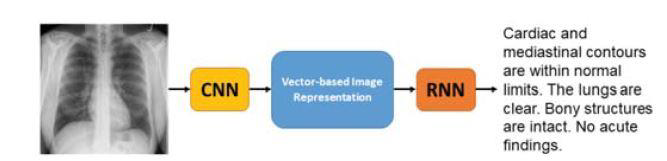
\includegraphics[width=7cm,height=7cm,keepaspectratio]{Encoder-Decoder}
\end{center}

Il codificatore ha la forma di una rete neurale convoluzionale (CNN) che codifica le immagini DICOM, mentre il decodificatore è una rete neurale ricorrente a più stadi (RNN) che traduce le caratteristiche dell'immagine medica in un referto radiologico.\\
In questo caso andiamo quindi a creare un framework codificatore-decodificatore, le caratteristiche dell'immagine globale vengono prima estratte utilizzando la CNN e quindi inserite in un LSTM (Long short-term memory che è un'architettura di rete neurale ricorrente artificiale utilizzata nel campo dell'apprendimento profondo) per generare una sequenza di parole. Quando si applica la struttura del codificatore-decodificatore alla generazione di referti di radiologia, l'attività può essere considerata come la traduzione di immagini mediche in referti di radiologia.\\
La figura seguente mostra il diagramma del nostro approccio alla generazione di report da immagini mediche. Per generare referti radiologici da immagini mediche, ci viene fornita un'immagine di inputi $I$ e il modello dovrebbe generare una sequenza di parole $y = (y_1, y_2, . . . ,y_N)$, dove $y$ denota la descrizione sotto forma di referto radiologico e $y_1 . . .y_N$ denotano le parole nella relazione.\\
Dato un set di allenamento $D = (I, y)$ che consiste in $(I, y)$ coppie, dove $I$ rappresenta una data immagine medica e $y$ rappresenta un referto radiologico accompagnato per l'immagine sotto di $y = (y_1, y_2, . . . ,y_N)$, addestriamo il modello rispetto ai suoi parametri $\theta$ al fine di massimizzare un modello probabilistico $p_{\theta}(y_1, y_2, . . . , y_N|I)$

\begin{center}
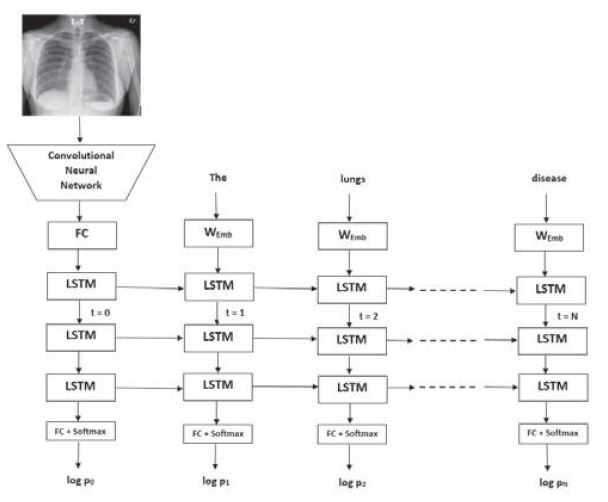
\includegraphics[width=7cm,height=7cm,keepaspectratio]{LSTM}
\end{center}

\subsubsection{Encoder}
Le reti neurali convoluzionali (CNN) sono comunemente utilizzate per le rappresentazioni di immagini in quanto hanno la capacità di catturare caratteristiche a vari livelli di astrazione. Le CNN hanno mostrato prestazioni all'avanguardia nella classificazione delle immagini e nel riconoscimento degli oggetti. I livelli in una CNN includono livelli convoluzionali, livelli di pooling e livelli completamente connessi. 
In questo studio, viene utilizzato il modello Inception-v3 di Google come codificatore perché ha una struttura significativamente più profonda e, grazie ai blocchi di Inception, apprende una rappresentazione semanticamente ricca delle immagini

\subsubsection{Decoder}
Le reti neurali ricorrenti (RNN) sono reti neurali specializzate che eccellono nell'apprendimento e nell'elaborazione di dati sequenziali come testo e parlato. Gli RNN sono generalmente addestrati dalla retropropagazione nel tempo, il che può portare a problemi di gradienti evanescenti ed esplosivi. Due degli RNN più popolari e importanti che superano questi problemi sono Long-Short Term Memory (LSTM) e Gated Recurrent Unit (GRU).

\subsection{Formazione del modello}
Il framework, quindi, è costituito da un codificatore che trasforma l'immagine grezza in una rappresentazione vettoriale e un decodificatore che trasforma il vettore dell'immagine codificata in una sequenza di parole.\\
In questo framework della rete neurale, una CNN viene solitamente impiegata come codificatore per estrarre una rappresentazione globale di immagini e il decodificatore è solitamente un RNN che modella il $p(S_t|I, S_0, S_1, . . . ,S_{t-1})$, e genera le frasi corrispondenti.\\
L'obiettivo generale del framework del codificatore-decodificatore è trovare la sequenza di parole (frasi) più probabile che descriva una data immagine. Durante l'addestramento, vogliamo trovare il modello $\theta^*$ che soddisfa l’equazione 1:

\begin{equation}
{\displaystyle \theta^* =  \sum\limits_{(I, S)} \log p(S | I; \theta)}
\end{equation}

dove $\theta$ sono i parametri del modello, $I$ è l'immagine medica di input, e $S$ è il rapporto di verità fondamentale corrispondente all'immagine. La probabilità della descrizione corretta $S$ per una data immagine $I$ può essere modellato come la probabilità congiunta sulle sue parole $S_0, S_1, … ,S_{t-1}$ come indicato nell'equazione 2:

\begin{equation}
{\displaystyle \log p(S|I) =  \sum\limits_{t = 0}^{N} \log p(S_t | I, S_0, S_1, ..., S_{t-1})}
\end{equation}

dove $S_0$, $S_1$, $S_{t-1}$ denota le parole nell'immagine descrizione. $S_0$ denota uno speciale $<start>$ token e $S_N$ denota uno speciale $<end>$ token.\\
La figura seguente mostra il diagramma schematico di una cella LSTM:

\begin{center}
\includegraphics[width=7cm,height=7cm,keepaspectratio]{diagram_LSTM}
\end{center}


\subsection{Analisi dei risultati e miglioramento}
Text

\subsection{Distribuzione}
Text

\section{Analisi}
In questa fase di analisi ho cercato di confrontare alcuni casi che ho trovato in letteratura, sono andato alla ricerca di quali potessero essere le invarianti e le versatilità tra loro in modo da centrare il nostro obiettivo.\\
\\
La cosa principale che è comune a tutti è il la struttura dati: set di dati formato sempre  da immagine DICOM e/o annotazione.\\
Ovviamente alcuni input devono essere scartati perché non presentano le caratteristiche di cui abbiamo bisogno.\\
Per estrarre le caratteristiche dall’immagine viene sempre utilizzata un CNN per le sue elevate prestazioni nel riconoscimento delle immagini. La capacità delle CNN di apprendere complesse relazioni spaziali e
imparare modelli basati su pixel sottili e intricati li rendono perfetti strumento per apprendere dalle immagini radiologiche. \\
\\
Per quanto riguarda l'estrazione del testo, invece, le tecniche di elaborazione del linguaggio naturale (NLP) possono essere una chiave per analizzare con successo i referti radiologici per estrarre risultati e raccomandazioni clinicamente importanti. La programmazione neuro-linguistica (PNL) ha già mostrato il potenziale per automatizzare il compito di classificare i report di imaging in un modo che potrebbe informare le decisioni relative all'utilizzo e all'adeguatezza dell'imaging medico [11-13, Comparative].\\
Una classe di architetture di reti neurali, le reti neurali ricorrenti (RNN), ha recentemente attirato molta attenzione da parte dei ricercatori per la modellazione di sequenze e ha dimostrato di funzionare bene nella risoluzione di vari compiti di PNL grazie alla loro capacità di gestire input di lunghezza variabile e uscita [27].\\
Sebbene RNN sia teoricamente un modello potente per codificare informazioni sequenziali, in pratica spesso soffre dei problemi di sfumatura/esplosione del gradiente mentre apprende le dipendenze a lungo raggio [33]. Le reti LSTM [34] e GRU [35] sono note per essere rimedi efficaci a questi problemi.\\
Le estensioni più popolari di RNN sono, appunto, Long Short-Term Memory (LSTM) [77] e la Gated Recurrent Unit (GRU) [78]. La memoria a lungo termine utilizza blocchi di memoria per salvare lo stato temporale della rete e porte per monitorare il flusso di informazioni. D'altra parte, GRU è una forma più leggera di RNN rispetto a LSTM in termini di topologia, spese di calcolo e complessità. Al momento, i ricercatori devono scegliere tra il modello più veloce offerto da GRU che necessita di meno parametri o il modello più performante fornito da LSTM che contiene dati sufficienti e potenza di calcolo [8].\\
\\
In generale, lo sviluppo di algoritmi di intelligenza artificiale generalizzabili nell'imaging medico richiede set di dati statisticamente alimentati nell'ordine di centinaia di migliaia o milioni, il che è problematico, data la scarsa disponibilità
dei dati.\\
In alcuni modelli, proprio per questa limitazione, viene eseguito un aumento dei dati di addestramento.\\
Una soluzione parziale per questo problema può essere l'apprendimento semisupervisionato. Sono necessari
set di dati completamente annotati per l'apprendimento supervisionato, mentre l'apprendimento semisupervisionato
utilizza una combinazione di immagini annotate e non annotate per addestrare un algoritmo (67,68).
L'apprendimento semi-supervisionato può consentire un numero limitato di casi annotati; tuttavia, sono ancora 
necessari grandi set di dati di immagini non annotate.
Un'altra potenziale soluzione futura per aumentare la dimensione del campione di dati potrebbe essere la generazione di dati 
sintetici attraverso reti generative avversarie (69). Le reti generative avversarie hanno il potenziale per sintetizzare un numero
illimitato di immagini realistiche di alta qualità che possono essere aggiunte ai set di dati di addestramento per lo sviluppo di 
algoritmi di rilevamento e classificazione. Tuttavia, sono disponibili prove limitate, specialmente quando sono presenti anomalie nelle immagini.
L'aumento dell'immagine sarebbe preferibile per aumentare il livello di robustezza del modello. Ovviamente, l'aumento delle immagini si traduce in un aumento del numero di set di dati per la formazione e potrebbe esserci il rischio del problema di sovradattamento.\\
Anche se viene esaminato lo stesso paziente, le immagini non sarebbero identiche tra gli esami a causa di lievi differenze di posizionamento. 
Pertanto, l'uso di immagini ruotate o spostate parallelamente renderebbe il modello robusto per lievi differenze nelle posizioni del paziente. A volte vengono utilizzate anche immagini speculari. L'uso di immagini con rumore aggiunto sarebbe utile per rendere il modello robusto per diversi gradi di rumore dell'immagine.\\
\\
Come già detto precedentemente, un modello potrebbe differire da un altro anche per le strategie di campionamento del set di dati:
\begin{itemize}
    \item Addestramento, convalida e test
    \item Convalida incrociata k-fold
\end{itemize}
Anche se il primo è quello più utilizzato, poiché il processo di formazione richiede un'enorme quantità di calcoli.\\
\\
Inoltre è possibile trovare alcuni modelli (ex: nel framework r.AID.ologist) concepiti come modello di ragionamento basato sui casi (Case-Based Reasoning - CBR), alimentato da diversi modelli di deep learning che sono stati inclusi per migliorarne le prestazioni, oltre a fornire funzionalità aggiuntive.
Sebbene CBR sia integrato come un ciclo continuo, le sue sottoparti sono progettate per essere completamente modulari, quindi possono essere facilmente sostituite per adattarsi a nuovi dati.

Il ragionamento basato su casi (CBR) è il processo di risoluzione di nuovi problemi basandosi sulle soluzioni di problemi anteriori ed è stato formalizzato, per il ragionamento automatico, come un processo suddiviso in quattro fasi:
\begin{enumerate}
\item Recupero: Dato un problema, recuperare in memoria dei casi rilevanti (ricordi) per risolverlo. Un caso è composto da un problema, la soluzione e tipicamente alcune annotazioni su come si è arrivati alla soluzione.
\item Riutilizzo: Mappare la soluzione del caso precedente al problema attuale. Ciò può comportare alcune modifiche al caso precedente per adattarlo al caso attuale.
\item Revisione: Avendo mappato la soluzione precedente al caso attuale, bisogna provare la nuova soluzione (nel mondo reale o con una simulazione) e, se necessario rivedere la nuova soluzione.
\item Conservazione: Dopo che la soluzione è stata adattata al problema attuale, memorizzare l'esperienza come nuovo caso.
\end{enumerate}


\chapter{Demand forecasting}
La previsione della domanda è uno dei problemi principali delle catene di approvvigionamento. Mira ad ottimizzare le scorte, ridurre i costi e aumentare le vendite, i profitti e la fedeltà dei clienti. A tal fine, i dati storici possono essere analizzati per migliorare la previsione della domanda utilizzando vari metodi come tecniche di apprendimento automatico, analisi di serie temporali e modelli di deep learning.\\
In questo studio viene analizzato il workflow della previsione della domanda con i relativi modelli. 

\section{Overview}
Poiché la concorrenza aumenta di giorno in giorno tra i rivenditori sul mercato, le aziende stanno concentrando più tecniche di analisi predittiva per ridurre i costi e aumentare la produttività e il profitto.\\
Esistono diversi tipi di previsione della domanda:
\begin{itemize}
    \item A breve termine (viene effettuato per un periodo più breve da 3 mesi a 12 mesi). 
    \item Da medio a lungo termine (in genere viene effettuato da più di 12 mesi a 24 mesi in anticipo (36-48 mesi in alcune attività)).
    \item Livello aziendale interno (questo tipo di previsione si occupa delle operazioni interne dell'azienda come categoria di prodotto, divisione vendite, divisione finanziaria e gruppo di produzione. Ciò include previsioni di vendita annuali, stima di COGS, margine di profitto netto, flusso di cassa, ecc.)
    \item Passivo (Si effettua per imprese stabili con piani di crescita molto conservativi. Semplici estrapolazioni di dati storici vengono effettuate con ipotesi minime.)
    \item Attivo (viene eseguito per ridimensionare e diversificare le aziende con piani di crescita aggressivi in termini di attività di marketing, espansione del portafoglio di prodotti e considerazione delle attività della concorrenza e dell'ambiente economico esterno).
\end{itemize}

I rivenditori in diversi settori sono alla ricerca di soluzioni automatizzate di previsione della domanda e rifornimento che utilizzino big data e tecnologie di analisi predittiva [3]. \\
I metodi di previsione tradizionali si basano su approcci di previsione basati su serie temporali. Questi approcci di previsione prevedono la domanda futura in base a dati di serie temporali storiche, ovvero una sequenza di punti dati misurati a intervalli successivi nel tempo. Questi metodi utilizzano un numero limitato di dati storici di serie temporali relativi alla domanda. Negli ultimi due decenni, I modelli di data mining e machine learning hanno attirato maggiore attenzione e sono stati applicati con successo alla previsione delle serie temporali.\\\
I metodi di previsione dell'apprendimento automatico possono utilizzare una grande quantità di dati e funzionalità correlate alla domanda e prevedere la domanda e i modelli futuri utilizzando diversi algoritmi di apprendimento. Tra molti metodi di apprendimento automatico, i metodi di deep learning (DL) sono diventati molto popolari e sono stati recentemente applicati a molti campi come il riconoscimento di immagini e parole, l'elaborazione del linguaggio naturale e la traduzione automatica.
I metodi DL hanno prodotto previsioni e risultati migliori, rispetto ai tradizionali algoritmi di apprendimento automatico in molte ricerche. 

\section{Workflow}

\subsection{Raccolta dati}
Il primo compito quando si avvia il progetto di previsione della domanda è fornire al cliente informazioni significative. Il processo include i seguenti passaggi:
\begin{enumerate}
    \item Raccogliere i dati disponibili
    \item Esaminare brevemente la struttura dei dati, l'accuratezza e la coerenza
    \item Eseguire alcuni test e progetti pilota sui dati
    \item Guardare attraverso un riepilogo statistico
\end{enumerate}

In questo caso studio il tipo di dato può essere molto differente in base all'obiettivo aziendale. Distinguiamo i dati in:
\begin{itemize}
    \item Strutturati
    \item Non strutturati
\end{itemize}

Nei dati strutturati possiamo trovare dati interni come i dati di vendita e-commerce, le transazioni di vendita, gli ordini d'acquisto, le proprie informazioni POS e dati esterni come tempo metereologico, spedizioni/ricevute del negozio del cliente, le informazioni POS cliente e dati sindacati di terze parti.\\
Nei dati non strutturati possiamo trovare dati interni come siti web, recensioni, campagne di marketing, app, dispositivi in negozio e dati esterni come social media, stream di click, IoT, dispositivi di geolocalizzazione, video, linguaggio naturale.\\

\subsection{Comprensione e preelaborazione dei dati}
Indipendentemente da ciò che vorremmo prevedere, la qualità dei dati è una componente fondamentale di una previsione accurata della domanda.

\subsubsection{Parametri di qualità dei dati}
Quando si costruisce un modello di previsione, i dati vengono valutati in base ai seguenti parametri:
\begin{itemize}
    \item Consistenza
    \item Precisione
    \item Validità
    \item Rilevanza
    \item Accessibilità
    \item Completezza
    \item Detalizzazione
\end{itemize}

\subsubsection{Preelaborazione dei dati}
In realtà, i dati raccolti dalle aziende spesso non sono ideali. Questi dati di solito devono essere puliti, analizzati per lacune e anomalie, verificati per pertinenza e ripristinati.
La preelaborazione può essere applicata in tre forme: adeguamenti stagionali, log o trasformazioni di potenza e rimozione della tendenza.
\begin{itemize}
    \item Dati originali: non viene applicata alcuna preelaborazione.
    \item Trasformazione dei dati: Ai dati originali viene applicato il log o la trasformazione di potenza Box-Cox [66] per ottenere la stazionarietà nella varianza.
    \item Destagionalizzazione dei dati: i dati sono considerati stagionali se esiste un coefficiente di autocorrelazione significativo al lag 12. In tal caso i dati vengono destagionalizzati utilizzando il classico approccio di decomposizione moltiplicativa [39]. L'addestramento dei pesi ML, o l'ottimizzazione dei metodi statistici, viene successivamente effettuato sui dati destagionalizzati. I pronostici ottenuti vengono poi ristagionali per determinare i pronostici finali. Ciò non avviene nel caso dei metodi ETS e ARIMA poiché includono modelli stagionali, selezionati utilizzando test relativi e criteri informativi che si occupano direttamente della stagionalità e della complessità del modello.
    \item Detrending dei dati: viene eseguito un test di Cox-Stuart [67] per stabilire se sia necessario utilizzare un trend lineare deterministico, o in alternativa un primo differenziamento, per eliminare il trend dai dati e ottenere la stazionarietà nella media.
    \item Combinazione dei tre precedenti: i vantaggi delle singole tecniche di pre-elaborazione vengono applicati simultaneamente per regolare i dati originali. Al fine di accelerare i calcoli, prima determiniamo la migliore alternativa di pre-elaborazione per migliorare le prestazioni di previsione post-campione in un passo avanti del metodo MLP (il più popolare tra quelli ML) e poi applichiamo quella ai restanti modelli ML.
\end{itemize}

Una volta che i dati sono stati puliti, generati e verificati per pertinenza, vengono strutturati in un modulo completo.\\
La comprensione dei dati è il compito successivo una volta completate la preparazione e la strutturazione. Non è ancora un modello, ma è un modo eccellente per comprendere i dati tramite la visualizzazione. 
Prima di iniziare a creare modelli, bisogna dividere il set di dati per l'addestramento, la convalida e il test.


\subsection{Costruzione del modello}
Non esistono algoritmi di previsione "taglia unica". Spesso, le funzionalità di previsione della domanda consistono in diversi approcci di apprendimento automatico. La scelta dei modelli di apprendimento automatico dipende da diversi fattori, come l'obiettivo aziendale, il tipo di dati, la quantità e la qualità dei dati, il periodo di previsione, ecc.\\
Mostreremo innanzitutto  i metodi statisti tradizionali e poi ci concentreremo su quelli utilizzando il ML, in particolare sull'approccio per serie temporali, che è quello più utilizzato.

Nei modelli di previsione delle serie temporali, l'approccio classico consiste nel raccogliere dati storici, analizzare questi dati sottostanti e utilizzare il modello per prevedere il futuro [28]. Questi algoritmi sono algoritmi di previsione comunemente usati nel dominio di previsione della domanda di serie temporali.

\subsubsection{Perceptron multistrato (MLP)}
Il perceptron multistrato (spesso chiamato semplicemente rete neurale) è forse l'architettura di rete più popolare oggi in uso sia per la classificazione che per la regressione (Bishop, 1995). Il MLP è dato come segue:

\begin{equation}
{\displaystyle \hat{y} = v_0 + \sum\limits_{j=1}^{NH} v_jg(w_{j}^{T}x')} ,
\end{equation}

dove $x'$ è il vettore di input $x$, aumentato di 1, cioè $ x' = (1, x^T )^T  $, $w_j$  è il vettore dei pesi per j-esimo nodo nascosto, $v_0, v_1, ..., v_{NH}$ sono i pesi per l'output nodo e $\hat{y}$ è l'output di rete. La funzione g rappresenta l'output del nodo nascosto, ed è data in termini di una funzione di schiacciamento, ad esempio la funzione logistica:
$g(u) = 1/(1 + exp(-u))$. 
Un modello correlato nella letteratura econometrica è il modello di autoregressione a transizione graduale che si basa anche sulla costruzione di funzioni lineari e transizioni di funzioni logistiche (Medeiros e Veiga, 2000; van Dijk et al., 2002).
L'MLP è un modello fortemente parametrizzato e selezionando il numero di nodi nascosti NH possiamo controllare la complessità del modello. La svolta che ha dato credito alla capacità delle reti neurali è la proprietà di approssimazione universale (Cybenko, 1989; Funahashi, 1989; Hornik et al., 1989; Leshno et al., 1993). In determinate condizioni blande sulle funzioni del nodo nascosto g , ogni data funzione continua su un insieme compatto può essere approssimata il più vicino possibile a quella data arbitrariamente utilizzando una rete con un numero finito di nodi nascosti. Sebbene questo sia un risultato rassicurante, è fondamentale evitare un'eccessiva parametrizzazione, specialmente nelle applicazioni di previsione che in genere hanno una quantità limitata di dati altamente rumorosi. La selezione del modello (attraverso la selezione del numero di nodi nascosti) ha quindi suscitato molto interesse nella letteratura sulle reti neurali (vedi Anders e Korn, 1999; Medeiros et al., 2006 per esempio). Viene usata una procedura di convalida K-fold per selezionare il numero di nodi nascosti.
Per ottenere i pesi, viene definito l'errore quadratico medio e i pesi vengono ottimizzati utilizzando tecniche di gradiente. Il metodo più noto, basato sul concetto di discesa più ripida, è l'algoritmo di backpropagation. Un metodo di ottimizzazione del secondo ordine chiamato Levenberg Marquardt è generalmente noto per essere più efficiente dell'algoritmo di retropropagazione di base.


\subsubsection{Rete neurale bayesiana (BNN)}
Una rete neurale bayesiana (BNN) è una rete neurale progettata sulla base di una formulazione probabilistica bayesiana (MacKay, 1992a,b). In quanto tali, i BNN sono correlati al concetto di statistica classica della stima dei parametri bayesiani e sono anche correlati al concetto di regolarizzazione come nella regressione della cresta. Le BNN hanno goduto di un'ampia applicabilità in molte aree come l'economia/finanza (Gencay e Qi, 2001) e l'ingegneria (Bishop, 1995). L'idea di BNN è di trattare i parametri oi pesi di rete come variabili casuali, obbedendo a una distribuzione a priori. Questa distribuzione è progettata in modo da favorire modelli a bassa complessità, cioè modelli che producono accoppiamenti lisci. Una volta osservati i dati, viene valutata la distribuzione a posteriori dei pesi e può essere calcolata la previsione della rete. Le previsioni rifletteranno quindi sia l'aspetto di levigatezza imposto dal precedente sia l'aspetto di accuratezza del fitness imposto dai dati osservati.\\
Un concetto strettamente correlato è l'aspetto della regolarizzazione, per cui la seguente funzione obiettivo è costruita e minimizzata

\begin{equation}
{\displaystyle J =\alpha E_D + (1 - \alpha)E_W}
\end{equation}

dove $E_D$ è la somma dei quadrati degli errori nelle uscite di rete, $E_W$ è la somma dei quadrati dei parametri di rete (cioè i pesi) ed è il parametro di regolarizzazione.
Per l'approccio bayesiano, la scelta tipica del priore (credenze iniziali su un evento in termini di distribuzione di probabilità) è la seguente densità normale che dà più peso ai valori dei parametri di rete più piccoli

\begin{equation}
{\displaystyle p(w) = \left( \frac{1 - \alpha}{\pi} \right)^{\frac{L}{2}} e^{-(1 - \alpha)E_W}}
\end{equation}

dove $L$ indica il numero di parametri (pesi). Il posteriore è quindi dato da

\begin{equation}
{ \displaystyle p(w \vert D, \alpha) = \frac{p(D \vert w, \alpha)p(w, \alpha)}{p(D, \alpha)} }
\end{equation}

dove $D$ rappresenta i dati osservati. Assumendo errori normalmente distribuiti, la densità di probabilità dei dati dati i parametri può essere valutata come

\begin{equation}
{ \displaystyle p(D \vert w, \alpha) = \left( \frac{\alpha}{\pi} \right)^{\frac{M}{2}}  e^{-(1 - \alpha)E_D} }
\end{equation}

dove $M$ è il numero di punti dati di addestramento. Sostituendo le espressioni per le densità in (3) e (5) in (4), otteniamo

\begin{equation}
{ \displaystyle p(w \vert D, \alpha) = c exp(-J) }
\end{equation}

dove $c$ è una costante di normalizzazione. La costante di regolarizzazione $\alpha$ è anche determinata utilizzando concetti bayesiani, da

\begin{equation}
{ \displaystyle p(\alpha \vert D) = \frac{p(D \vert \alpha)p(\alpha)}{p(D)} }
\end{equation}

Entrambe le espressioni (6) e (7) dovrebbero essere massimizzate per ottenere rispettivamente i pesi ottimali e il parametro $\alpha$. Il termine $p(D \vert \alpha)$ in (7) è ottenuto da un'approssimazione quadratica di $J$ in termini di pesi e quindi integrando i pesi. 

\subsubsection{Reti neurali di regressione generalizzata (GRNN)}
Nadaraya e Watson hanno sviluppato questo modello (Nadaraya, 1964; Watson, 1964).
È comunemente chiamato stimatore Nadaraya-Watson o stimatore di regressione del kernel. Nella comunità del machine learning, viene in genere utilizzato il termine rete neurale di regressione generalizzata (o GRNN). Useremo quest'ultimo termine. Il modello GRNN è un modello non parametrico in cui la previsione per un dato punto dati $x$ è data dalla media degli output target dei punti dati di addestramento nelle vicinanze del dato punto $x$ (Hardle, 1990). La media locale è costruita pesando i punti in base alla loro distanza da $x$, usando alcune funzioni del kernel. La stima è solo la somma ponderata delle risposte osservate (o output target) data da

\begin{equation}
equation-one
\end{equation}

dove i pesi $w_m$ sono dati da

\begin{equation}
equation-two
\end{equation}

dove $y_m$ è l'output di destinazione per il punto dati di training $x_m$ e $K$ è la funzione del kernel. Abbiamo usato il tipico kernel gaussiano $formula$.
Il parametro $h$, chiamato larghezza di banda, è un parametro importante in quanto determina la levigatezza dell'adattamento, poiché aumentandolo o diminuendolo controllerà la dimensione della regione di levigatura.

\subsubsection{Regressione K-Nearest Neighbor (KNN)}
KNN è un metodo non parametrico che basa la sua previsione sugli output di destinazione dei $K$ vicini più vicini del dato punto di interrogazione (vedi Hastie et al., 2001). Nello specifico, dato un punto dati, calcoliamo la distanza euclidea tra quel punto e tutti i punti del training set. Quindi selezioniamo i punti dati di allenamento $K$ più vicini e impostiamo la previsione come media dei valori di output target per questi K punti. Quantitativamente parlando, sia $I(x)$ l'insieme di $K$ vicini più prossimi del punto $x$. Allora la previsione è data da

\begin{equation}
{\displaystyle \hat{y} = \frac{1}{K} \sum\limits_{m \in I(x)} y_m}
\end{equation}

dove di nuovo $y_m$ è l'output di destinazione per il punto dati di training $x_m$.
Naturalmente $K$ è un parametro chiave in questo metodo e deve essere selezionato con cura. Un $K$ grande porterà a un adattamento più fluido, e quindi a una varianza inferiore, ovviamente a scapito di un bias maggiore, e viceversa per un $K$ piccolo.

\subsubsection{Regressione del vettore di supporto (SVR)}
La regressione del vettore di supporto (Scholkopf e Smola, 2001; Smola e Scholkopf, 2003) è un metodo di successo basato sull'utilizzo di uno spazio di caratteristiche ad alta dimensione (formato trasformando le variabili originali) e penalizzando la conseguente complessità utilizzando un termine di penalità aggiunto alla funzione di errore. Consideriamo prima per l'illustrazione un modello lineare. Quindi, la previsione è data da

\begin{equation}
equation-one
\end{equation}

dove $w$ è il vettore del peso, $b$ è il bias e $x$ è il vettore di input. Sia $x_m$ e $y_m$ denotano, rispettivamente, l' m-esimo vettore di input di addestramento e output di destinazione, $m = 1, …, M$. La funzione di errore è data da 

\begin{equation}
equation-two
\end{equation}

Il primo termine nella funzione di errore è un termine che penalizza la complessità del modello. Il secondo termine è la funzione di perdita $\epsilon-insesitive$, definita come

\begin{equation}
equation-three
\end{equation}

Non penalizza gli errori sottostanti, consentendo un po' di spazio di manovra per lo spostamento dei parametri per ridurre la complessità del modello. Si può dimostrare che la soluzione che minimizza la funzione di errore è data da

\begin{equation}
equation-four
\end{equation}

dove $\alpha_m$ e $\alpha_m^\ast$ sono moltiplicatori di Lagrange. I vettori di addestramento che forniscono moltiplicatori di Lagrange diversi da zero sono chiamati vettori di supporto e questo è un concetto chiave nella teoria SVR. I vettori non di supporto non contribuiscono direttamente alla soluzione e il numero di vettori di supporto è una misura della complessità del modello (vedi Chalimourda et al., 2004; Cherkassky e Ma, 2004). Questo modello viene esteso al caso non lineare attraverso il concetto di kernel $K$, dando una soluzione

\begin{equation}
equation-five
\end{equation}

Un kernel comune è il kernel gaussiano. Assumiamo che la sua larghezza sia $\sigma K$ (la deviazione standard della funzione gaussiana).


\subsubsection{Rete Neurale Ricorrente (RNN)}
L'RNN semplice, noto anche come rete di Elman, ha una struttura simile all'MLP, ma contiene connessioni di feedback per tenere conto degli stati precedenti insieme all'input corrente prima di produrre l'output o gli output finali.
Questo viene fatto salvando una copia dei valori precedenti del livello contenente i nodi ricorrenti e utilizzandoli come input aggiuntivo per il passaggio successivo. A questo proposito, la rete può esibire un comportamento temporale dinamico per una sequenza temporale.
In questo studio il modello utilizzato per implementare la RNN è quello sequenziale. È composto da due livelli, uno nascosto contenente nodi ricorrenti e uno di output contenente uno o più nodi lineari. A causa degli elevati requisiti computazionali, non è stata utilizzata la convalida k-fold per scegliere l'architettura di rete ottimale per serie, ma piuttosto tre nodi di input e sei unità ricorrenti, che formano lo strato nascosto, per tutte le serie temporali del set di dati. 


\subsubsection{Rete neurale di memoria a lungo termine (LSTM)}
La rete LSTM è simile alla RNN discussa sopra ed è stata proposta per evitare il problema della dipendenza a lungo termine. Il vantaggio delle unità LSTM rispetto alle normali unità RNN è la loro capacità di conservare le informazioni per periodi di tempo più lunghi grazie alla loro architettura complessa che consiste in diverse porte con il potere di rimuovere o aggiungere informazioni allo stato dell'unità.
Simile a RNN, il modello utilizzato per implementare la rete LSTM è quello sequenziale composto da uno strato nascosto e uno di output. Allo stesso modo, a causa dell'elevato tempo di calcolo, l'architettura del modello è costituita da tre nodi di input, sei unità LSTM che formano lo strato nascosto e un singolo nodo lineare nello strato di output. La funzione di attivazione lineare viene utilizzata prima dell'uscita di tutte le unità e quella del sigmoide rigido per il passo ricorrente. 

\subsection{Formazione del modello}
Una volta sviluppati i modelli di previsione, è il momento di iniziare il processo di formazione. Quando si addestrano i modelli di previsione, i data scientist di solito utilizzano dati storici. Elaborando questi dati, gli algoritmi forniscono modelli addestrati pronti per l'uso.


\subsection{Validazione del modelllo}
Questo passaggio richiede l'ottimizzazione dei parametri del modello di previsione per ottenere prestazioni elevate. Utilizzando un metodo di ottimizzazione della convalida incrociata in cui il set di dati di training è suddiviso in dieci parti uguali. I data scientist addestrano modelli di previsione con diversi set di iperparametri. L'obiettivo di questo metodo è capire quale modello ha la previsione più accurata.


\subsection{Miglioramento}
Quando si ricercano le migliori soluzioni aziendali, gli scienziati dei dati di solito sviluppano diversi modelli di apprendimento automatico. Poiché i modelli mostrano diversi livelli di accuratezza, gli scienziati scelgono quelli che soddisfano meglio le loro esigenze aziendali. La fase di miglioramento prevede l'ottimizzazione dei risultati analitici. Ad esempio, utilizzando tecniche di insieme di modelli, è possibile ottenere una previsione più accurata. In tal caso, l'accuratezza viene calcolata combinando i risultati di più modelli di previsione.

\subsection{Distribuzione}
Questa fase presuppone l'integrazione dei modelli di previsione nell'uso della produzione. Si consiglia inoltre di impostare una pipeline per aggregare nuovi dati da utilizzare per le tue prossime funzionalità di intelligenza artificiale. Ciò può far risparmiare molto lavoro di preparazione dei dati in progetti futuri. In questo modo aumenta anche la precisione e la varietà di ciò che potresti essere in grado di prevedere.


\section{Analisi}
In questa fase di analisi ho cercato di confrontare alcuni casi che ho trovato in letteratura, sono andato a ricercare quali potessero essere le invarianti e le versatilità tra loro.
Le svariate applicazioni della previsione della domanda portano anche a svariati modelli utilizzabili e svariati modi di pretrattare i dati.\\
\\
I diversi modi di pretrattare i dati dipendono dal tipo di modello utilizzato, se si prende in considerazione la stagionalità verrà utilizzato un determinato modello con un set di dati con una determinata struttura,
se viene utilizzato un modello per serie temporali abbiamo bisogno che i dati abbiano un timestamp, e così via..\\
Allo stesso tempo nei problemi di classificazione, le prestazioni degli algoritmi di apprendimento dipendono principalmente dalla natura della rappresentazione dei dati [23].\\

Come visto in precedenza le modalità di pretrattamento dei dati sono molteplici:
\begin{itemize}
    \item Trasformazione dei dati (log o la trasformazione di potenza Box-Cox [66]).
    \item Destagionalizzazione dei dati.
    \item Detrending dei dati.
    \item Combinazione dei tre precedenti
\end{itemize}

Si è evidenziata inoltre la necessità non solo di considerare l'uso attento dei metodi di preparazione dei dati, ma di testare attivamente più combinazioni diverse di schemi di preparazione dei dati per un dato problema al fine di scoprire cosa funziona meglio, anche nel caso dei metodi classici.\\
\\
Un'altro passaggio che ho trovato in letteratura è la clusterizzazione dei dati.
\paragraph*{Clustering dei dati:}
Identificare e separare diversi modelli nei dati e utilizzare ciascuno di essi come set di dati indipendenti. Questo è noto come clustering e può essere ottenuto utilizzando algoritmi di apprendimento automatico.
Nell'apprendimento non supervisionato, un problema comune è identificare e classificare correttamente un certo numero di classi identiche (cluster) presenti nei dati (Bishop 2006). All'inizio, il numero di cluster, k, è solitamente sconosciuto. Trovarlo può essere ottenuto eseguendo l'algoritmo di clustering per diversi valori di k e valutando i risultati per ciascun valore.\\
Il numero ottimale di cluster è quello che ottimizza un determinato criterio, come la varianza tra osservazioni nello stesso cluster.
Complessivamente, il numero di cluster e il modo in cui vengono trovati, la formulazione della distanza e l'implementazione dell'algoritmo di clustering stesso sono reciprocamente influenzati e diverse combinazioni di essi produrranno risultati diversi.\\
Qui, l'analisi di clustering può essere utilizzata per verificare la stagionalità e altre relazioni tra i dati di input.\\
\\
Come visto in precedenza i modelli da poter utilizzare sono molteplici:
\begin{itemize}
    \item Perceptor multistrato (MLP)
    \item Rete neurale bayesiana (BNN)
    \item Reti neurali di regressione generalizzata (GRNN)
    \item Regressione K-Nearest Neighbor (KNN)
    \item Regressione del vettore di supporto (SVR)
    \item Rete Neurale Ricorrente (RNN)
    \item Rete neurale di memoria a lungo termine (LSTM)
\end{itemize}

\paragraph*{Ensemble Learning:}
Oltre a questi modelli discussi in precedenza c'è anche l'Ensemble Learning (EL), che è un'altra metodologia per aumentare le prestazioni del sistema.\\
Un sistema di insieme è composto da due parti:
\begin{itemize}
    \item generazione di insieme
    \item integrazione di insieme [4].
\end{itemize}
Nella parte di generazione dell'ensemble, viene generato un insieme diversificato di modelli di previsione di base utilizzando metodi o campioni diversi. Nella parte di integrazione, le previsioni di tutti i modelli vengono combinate utilizzando una strategia di integrazione.\\

Descrivo in breve un algoritmo in particolare che si approccia molto a questo caso, e si tratta dell'algoritmo Stacking:\\
Stacking o Stacked Generalization è un algoritmo di apprendimento automatico di insieme. Utilizza un algoritmo di meta-apprendimento per apprendere come combinare al meglio le previsioni di due o più algoritmi di apprendimento automatico di base.
Potremmo usare Stacking per combinare vari modelli e fare nuove previsioni.
L'architettura di un modello di impilamento (stacking model) coinvolge due o più modelli di base, spesso indicati come modelli di livello 0 e un meta-modello che combina le previsioni dei modelli di base indicati come modello di livello 1:
\begin{itemize}
    \item Modelli di livello 0 (modelli base): i modelli si adattano ai dati di addestramento e le cui previsioni vengono compilate.
    \item Modello di Livello 1 (Meta-Modello): modello che apprende come combinare al meglio le previsioni dei modelli base.
\end{itemize}
Il meta-modello è addestrato sulle previsioni fatte dai modelli di base su dati fuori campione. In altre parole, i dati non utilizzati per addestrare i modelli di base vengono inviati ai modelli di base, vengono effettuate previsioni e queste previsioni, insieme agli output previsti, forniscono le coppie di input e output del set di dati di addestramento utilizzato per adattarsi al meta-modello. Gli output dei modelli di base utilizzati come input per il meta-modello possono essere valori reali in caso di regressione e valori di probabilità, valori simili alla probabilità o etichette di classe in caso di classificazione.
La regressione a stack è una tecnica di apprendimento di insieme per combinare più modelli di regressione tramite un meta-regressore. I singoli modelli di regressione vengono addestrati in base al training set completo; quindi, il meta-regressore viene adattato in base agli output - meta-caratteristiche - dei singoli modelli di regressione nell'insieme.\\
\\
Dopo aver esaminato molti articoli in lettatura, gli studi fatti precedentemente forniscono importanti prove a sostegno del fatto che i metodi classici possono dominare la previsione di serie temporali, almeno sui tipi di problemi di previsione valutati.\\
La domanda più interessante e la sfida più grande è trovare le ragioni delle loro scarse prestazioni con l'obiettivo di migliorarne la precisione e sfruttarne l'enorme potenziale. Gli algoritmi di apprendimento dell'intelligenza artificiale hanno rivoluzionato un'ampia gamma di applicazioni in diversi campi e non c'è motivo per cui lo stesso non possa essere ottenuto con i metodi ML nella previsione. Quindi, si dovrebbe trovare come essere applicati per migliorare la loro capacità di prevedere in modo più accurato.
Gli autori di alcuni articoli fanno commenti su LSTM e RNN, che sono generalmente ritenuti l'approccio di deep learning per problemi di previsione di sequenza in generale, e in questo caso le loro prestazioni chiaramente scarse nella pratica.\\
\\
\emph{[...] one would expect RNN and LSTM, which are more advanced types of NNs, to be far more accurate than the ARIMA and the rest of the statistical methods utilized.}\\
\\
—  Makridakis S, Spiliotis E, Assimakopoulos V (2018) Statistical and Machine Learning forecasting methods: Concerns and ways forward. PLoS ONE 13(3): e0194889. https://doi.org/10.1371/journal.pone.0194889\\
\\
Dicendo anche che gli LSTM sembrano essere più adatti a adattare o sovradimensionare il set di dati di allenamento piuttosto che a prevederlo.\\
\\
\emph{Another interesting example could be the case of LSTM that compared to simpler NNs like RNN and MLP, report better model fitting but worse forecasting accuracy.}\\
\\
—  Makridakis S, Spiliotis E, Assimakopoulos V (2018) Statistical and Machine Learning forecasting methods: Concerns and ways forward. PLoS ONE 13(3): e0194889. https://doi.org/10.1371/journal.pone.0194889\\
\\

\paragraph*{Estrazione delle caratteristiche:}
Potrebbero esserci alcuni problemi a causa dell'enorme quantità di dati. Quando si prova ad utilizzare tutte le funzionalità di tutti i dati (es: i prodotti in ogni negozio con 155 funzionalità e 875 milioni di record), l'algoritmo di deep learning può impiegare persino giorni per completare il suo lavoro a causa della potenza di calcolo limitata. [An improved demand, page 5]\\
Quindi per ogni algoritmo è necessario ridurre il numero di caratteristiche e il tempo di calcolo. Per superare questo problema e accelerare le fasi di clustering e modellazione, potrebbe essere utilizzato PCA (Principal Component Analysis) come algoritmo di estrazione delle caratteristiche.\\
PCA è un algoritmo di riduzione delle dimensioni comunemente utilizzato che presenta le caratteristiche più significative. PCA trasforma ogni istanza del dato insieme di dati dallo spazio d dimensionale a un sottospazio dimensionale k in cui il nuovo insieme generato di k dimensioni è chiamato Componenti Principali (PC) [32]. Ciascuna componente principale è indirizzata a una varianza massima esclusa la varianza, contabilizzata in tutte le sue componenti precedenti. Di conseguenza, il primo componente copre la massima varianza e così via.\\
In breve, i Componenti Principali sono rappresentati come
\begin{equation}
    {\displaystyle PC_i = a_1X_1 + a_2X_2 + ...}
\end{equation}

dove $PC_i$ è l'$i$-esimo componente principale, $X_j$ è la $j$-esima caratteristica originale e $a_j$ è il coefficiente numerico per la caratteristica $X_j$.

\chapter{Frameworks}
Gli strumenti di orchestrazione del machine learning vengono utilizzati per automatizzare e gestire i workflows e l'infrastruttura della pipeline, con un'interfaccia semplice e collaborativa. Insieme alla gestione e alla creazione di workflows personalizzati e delle relative pipeline, questi strumenti ci aiutano anche a tracciare e monitorare i modelli per ulteriori analisi.
Gli strumenti di orchestrazione rendono il processo di machine learning più semplice, più efficiente e aiutano i data scientist e i team di machine learning a concentrarsi su ciò che è necessario, piuttosto che sprecare risorse cercando di identificare i problemi prioritari.\\
Cerchiamo, quindi, quali sono quei framework che meglio si adattano ai nostri case studies.

\section{MetaFlow}
Metaflow è una libreria Python di facile utilizzo che aiuta scienziati e ingegneri a creare e gestire progetti di data science reali, come nel caso della radiologia. Metaflow è stato originariamente sviluppato da Netflix per aumentare la produttività dei data scientist che lavorano su un'ampia varietà di progetti, dalle statistiche classiche al deep learning all'avanguardia.
Metaflow fornisce un'API unificata allo stack dell'infrastruttura necessario per eseguire progetti di data science, dal prototipo alla produzione, ma non presenta un'interfaccia grafica per visualizzare e gestire i flussi di lavoro.

\begin{center}
    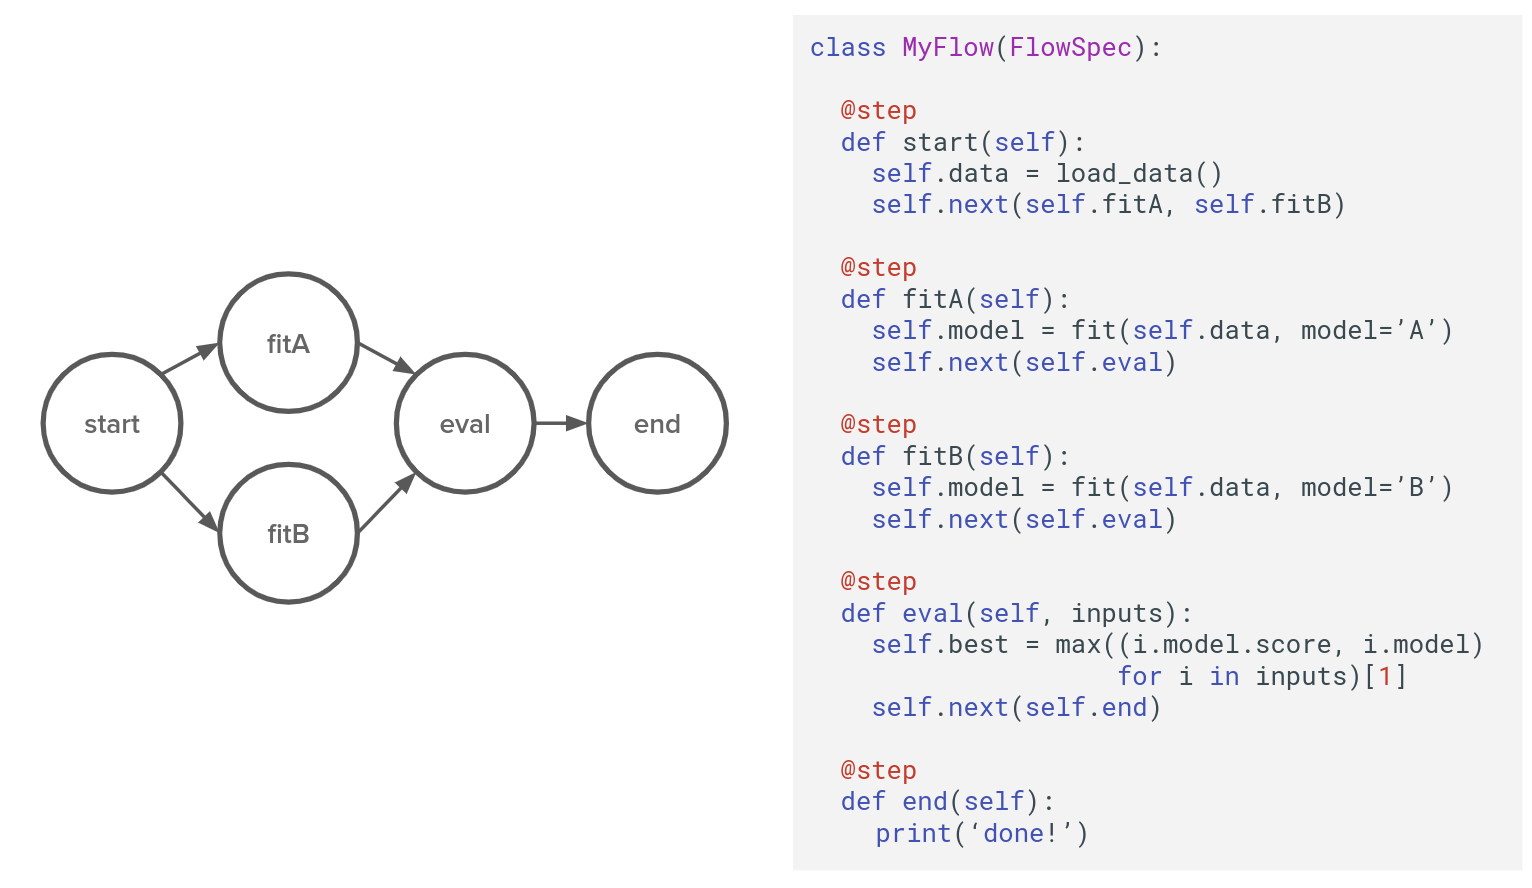
\includegraphics[width=7cm,height=7cm,keepaspectratio]{MetaFlow}
\end{center}

I data scientists possono strutturare il proprio flusso di lavoro come un grafico aciclico diretto di passaggi, come illustrato sopra. I passaggi possono essere codice Python arbitrario. In questo esempio ipotetico, il flusso addestra due versioni di un modello in parallelo e sceglie quella con il punteggio più alto. Anche per questo motivo si appresta al nostro caso. Per fare una predizione accurata, sarebbe conveniente addestrare varie versioni di un modello, o addiritura modelli differenti e scegliere il migliore.\\
In superficie, questo non sembra molto. Esistono molti framework esistenti, come Apache Airflow o Luigi, che consentono l'esecuzione di DAG costituiti da codice Python arbitrario. Il "problema" è nei molti dettagli accuratamente progettati di Metaflow: ad esempio, nota come nell'esempio sopra i dati e i modelli sono memorizzati come normali variabili di istanza Python. Funzionano anche se il codice viene eseguito su una piattaforma di calcolo distribuita, supportata da Metaflow per impostazione predefinita, grazie all'archivio di artefatti indirizzato al contenuto integrato di Metaflow. In molti altri framework, il caricamento e l'archiviazione degli artefatti è lasciato come esercizio per l'utente, che lo costringe a decidere cosa dovrebbe e non dovrebbe essere mantenuto. Metaflow rimuove questo sovraccarico cognitivo.
Metaflow è ricco di dettagli incentrati sull'uomo come questo, che mirano tutti ad aumentare la produttività dei data scientist.\\
\\
Metaflow segue il dataflow paradigm che modella un programma come un grafo diretto di operazioni. Questo è un paradigma naturale per esprimere le pipeline di elaborazione dei dati, in particolare l'apprendimento automatico.
Chiamiamo il grafico delle operazioni un flusso. Definisci le operazioni, chiamate passaggi, che sono nodi del grafico e contengono le transizioni ai passaggi successivi, che fungono da archi.\\
Metaflow imposta alcuni vincoli sulla struttura del grafico. Per cominciare, ogni flusso ha bisogno di un passaggio chiamato \emph{inizio} e un passaggio chiamato \emph{fine}. Un'esecuzione del flusso, che chiamiamo esecuzione, inizia all'\emph{inizio}. L'esecuzione ha esito positivo se il passaggio finale \emph{fine} termina correttamente.
Quello che succede tra l'\emph{inizio} e la \emph{fine} dipende da te.\\
Puoi costruire il grafico intermedio utilizzando una combinazione arbitraria dei seguenti tre tipi di transizioni supportati da Metaflow:
\begin{itemize}
    \item Linear 
    \item Branch
    \item Foreach
\end{itemize}

Questo framework si sposa molto bene con il nostro obiettivo perché:
\begin{itemize}
    \item Fornisce un'API altamente utilizzabile per strutturare il codice come flusso di lavoro, ovvero come grafico diretto dei passaggi (usabilità).
    \item Mantiene un'istantanea immutabile di dati, codice e dipendenze esterne necessarie per eseguire ogni passaggio (riproducibilità).
    \item Facilita l'esecuzione delle fasi in vari ambienti, dallo sviluppo alla produzione (scalabilità, prontezza alla produzione).
    \item Registra i metadati sulle precedenti esecuzioni e rendili facilmente accessibili (usabilità, riproducibilità).
\end{itemize}

\section{ZenML}
ZenML è un framework MLOps estensibile e open source per l'utilizzo di pipeline di Machine Learning pronte per la produzione, in modo semplice. Al suo interno, ZenML organizzerà le pipeline dei tuoi esperimenti dall'acquisizione dei dati alla suddivisione, pre-elaborazione, formazione, fino alla valutazione dei risultati e persino alla pubblicazione.
Sebbene esistano altre soluzioni di pipeline per gli esperimenti di Machine Learning, ZenML si concentra su quanto segue:
\begin{itemize}
    \item Semplicità.
    \item Riproducibilità.
    \item Integrazioni.
\end{itemize}

\subsection{Problemi risolti da ZenML}
ZenML risolve il problema di portare in produzione l'apprendimento automatico nei modelli. Dovresti usare ZenML se lotti con:
\begin{itemize}
    \item Riproduzione dei risultati della formazione in produzione.
    \item Gestione dei metadati ML, inclusi dati, codice e versionamento del modello.
    \item Ottenere (e mantenere) i modelli ML in produzione.
    \item Riutilizzare codici/dati e ridurre gli sprechi.
    \item Mantenimento della comparabilità tra i modelli ML.
    \item Ridimensionamento dell'addestramento/inferenza ML a set di dati di grandi dimensioni.
    \item Mantenimento della qualità del codice insieme alla velocità di sviluppo.
    \item Tenere il passo con il panorama degli strumenti ML in modo coerente.
\end{itemize}

Da aggiustare:\\
Nel caso del demand forecasting, come già detto in precedenza, potrebbe esserci la possibilità di ridurre il set di dati al fine di ridurre anche il tempo di addestramento. Questo framework consente un'ottimio ridimensionamento del set di dati.

Nel caso dell'AI in radiology, il riutilizzo del codice è fondamentale. Come abbiamo visto precedentemente per estrarre le caratteristiche da un immagine viene sempre utilizzata una CNN, a questo punto quel modulo potrà essere quasi sempre riutilizzato in tutti i casi di estrazione delle caratteristiche da un immagine.

\section{MLRun}
MLRun è un framework MLOps open source che offre un approccio integrativo alla gestione delle pipeline di machine learning dallo sviluppo iniziale allo sviluppo del modello fino alla distribuzione completa della pipeline in produzione. MLRun offre un comodo livello di astrazione per un'ampia varietà di stack tecnologici, consentendo ai data engineer e ai data scientist di definire la funzionalità e i modelli.\\
L'architettura MLRun
\begin{center}
    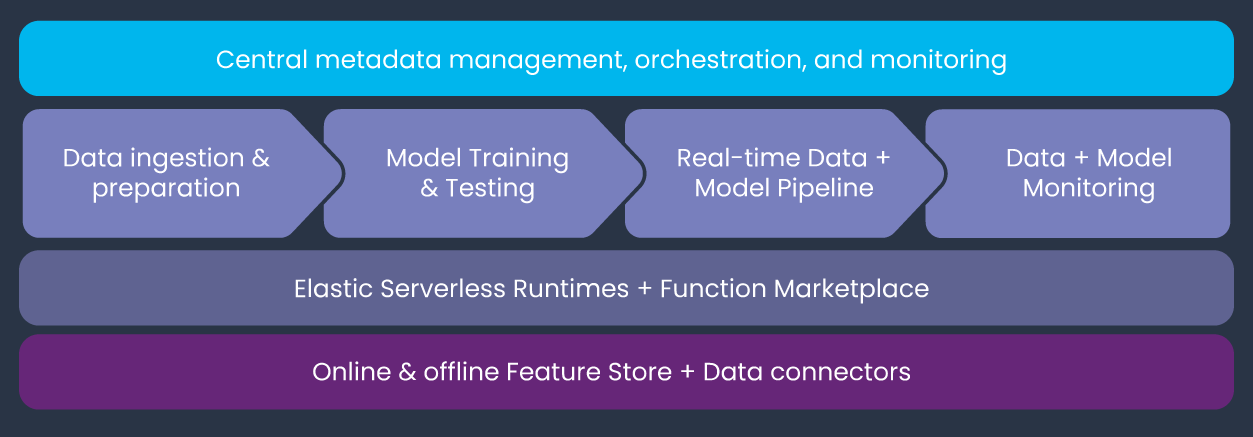
\includegraphics[width=7cm,height=7cm,keepaspectratio]{MLRun}
\end{center}

\subsection{Vantaggi chiave}
MLRun offre i seguenti vantaggi chiave:

\begin{itemize}
    \item Implementazione rapida del codice nelle pipeline di produzione
    \item Ridimensionamento elastico di carichi di lavoro batch e in tempo reale
    \item Gestione delle funzionalità: acquisizione, preparazione e monitoraggio
    \item Funziona ovunque: il tuo IDE locale, multi-cloud o on-premise
\end{itemize}


Per garantire efficienza e scalabilità, è necessario implementare il parallelismo quando possibile. MLRun supporta questo utilizzando due meccanismi:

\begin{enumerate}
    \item Clustering: eseguire il codice su un motore di elaborazione distribuito (come Dask, Spark o Horovod).
    \item Bilanciamento del carico/partizionamento: dividere (partizionare) il lavoro tra più lavoratori.
\end{enumerate}

Le funzioni e le attività MLRun possono accettare iperparametri o elenchi di parametri, distribuire molti worker paralleli e suddividere il lavoro tra i worker distribuiti. L'implementazione del parallelismo è lasciata al runtime. Ogni runtime può avere il proprio metodo di esecuzione delle attività simultanee.\\
MLRun supporta il parallelismo. Ad esempio, il codice seguente mostra come utilizzare gli iperparametri per eseguire l'attività di addestramento del modello XGBoost dall'esempio nella sezione precedente (xgb\_train) con diverse combinazioni di parametri:

\begin{lstlisting}
parameters = {
    "eta":       [0.05, 0.10, 0.20, 0.30],
    "max_depth": [3, 4, 5, 6, 8, 10],
    "gamma":     [0.0, 0.1, 0.2, 0.3],
    }

task = NewTask(handler=xgb_train, out_path='/User/mlrun/data').with_hyper_params(parameters, 'max.accuracy')
run = run_local(task)
\end{lstlisting}

Questo codice mostra come indicare a MLRun di eseguire la stessa attività mentre si scelgono i parametri da più elenchi (ricerca a griglia). MLRun quindi registra tutte le esecuzioni, ma contrassegna solo l'esecuzione con perdita minima come risultato selezionato.\\
Ed è proprio per questo che è un ottimo candidato per il nostro scopo. Data la mole di dati, per quanto riguarda il demand forecasting, il parallelismo rappresenta un ottima soluzione al problema di allenare una rete con tantissimi dati, altrimenti ci vorrebbero addiritura giorni.\\
\\
MLRun ha anche un'interfaccia utente grafica (MLRun Dashbord) per lavorare e visualizzare i dati
\begin{center}
    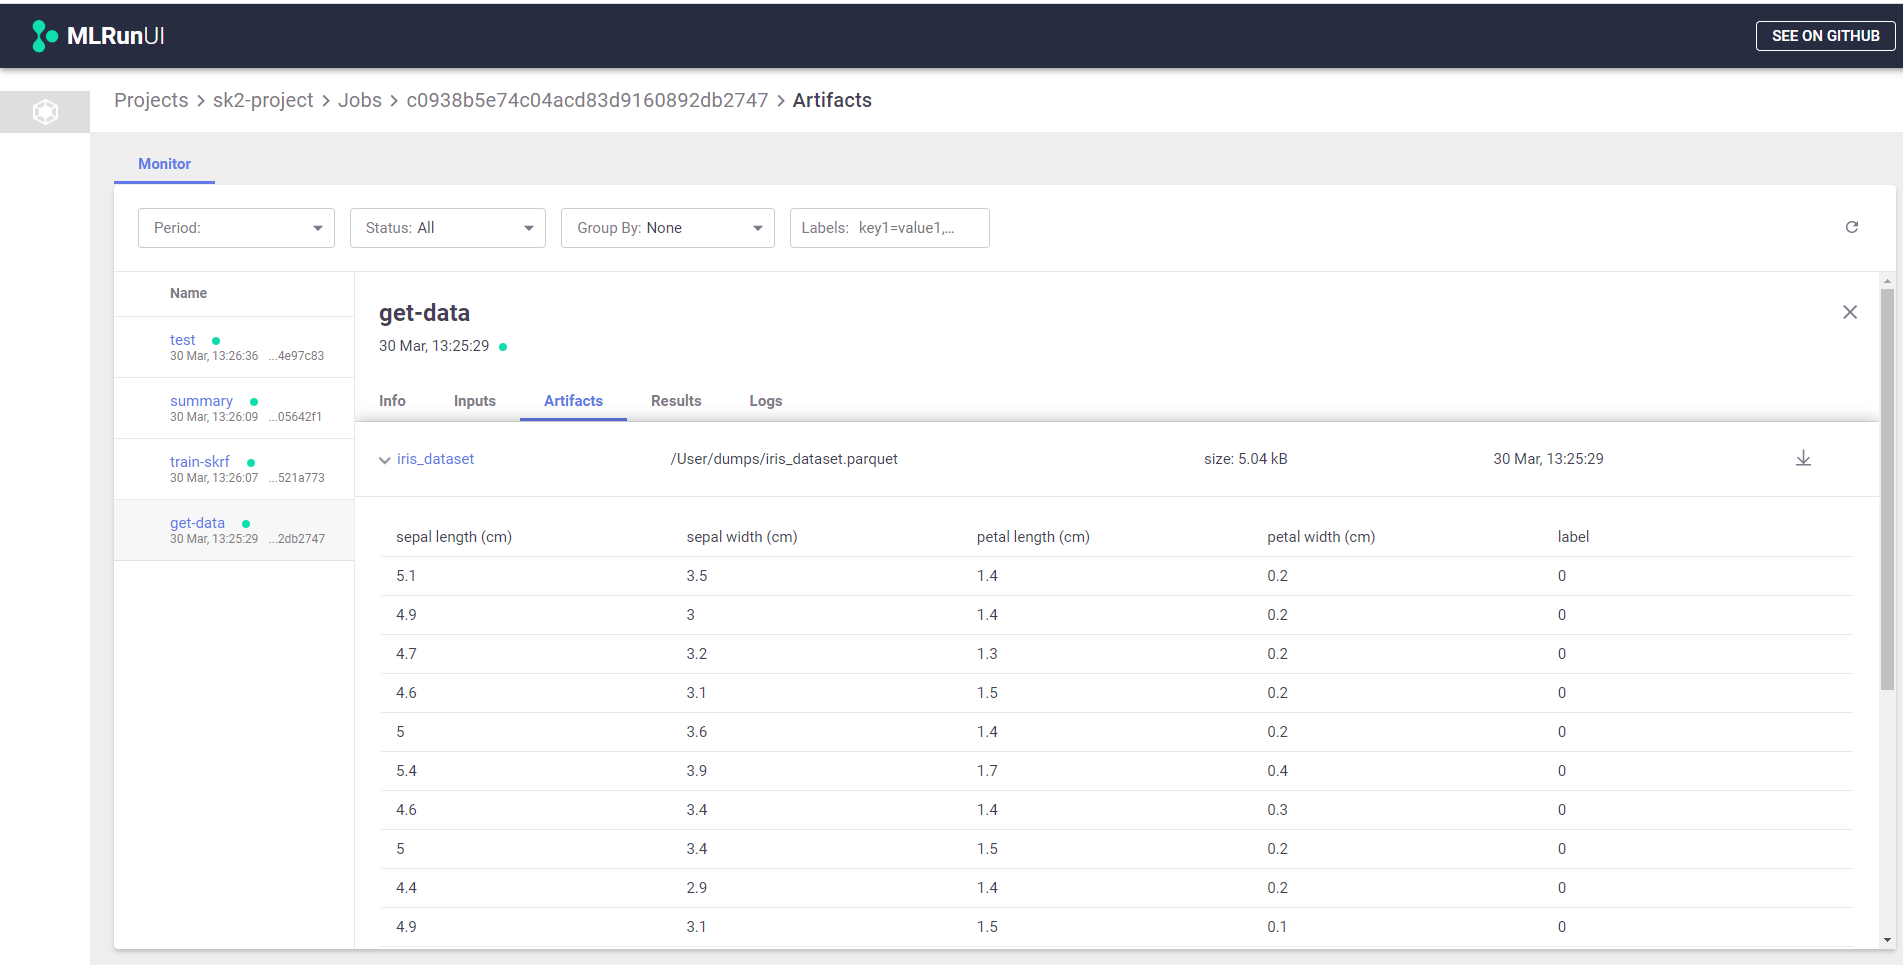
\includegraphics[width=15cm,height=15cm,keepaspectratio]{MLRun Dashbord}
\end{center}

\chapter{Conclusioni}


 





















\end{document}